\documentclass[a4paper,14pt]{extarticle}
\usepackage[utf8]{inputenc}
\usepackage[russian]{babel}
\usepackage{graphicx}
\usepackage[top=0.8in, bottom=0.8in, left=0.8in, right=0.8in]{geometry}
\usepackage{pgfplots}
\usepackage{amsmath}
\usepackage{setspace}
\usepackage{titlesec}
\usepackage{float}
\usepackage{chngcntr}
\usepackage{pgfplots}
\usepackage{amsfonts}
\usepackage{pgfplotstable}
\usepackage{multirow}
\usepackage{karnaugh-map}
\usepackage{tikz,xcolor}

\titleformat{\section}[hang]
  {\bfseries}
  {}
  {0em}
  {\hspace{-0.4pt}\large \thesection\hspace{0.6em}}
  
  
\titleformat{\subsection}[hang]
  {\bfseries}
  {}
  {0em}
  {\hspace{-0.4pt}\large \thesubsection\hspace{0.6em}}

%\linespread{1.3} % полуторный интервал
%\renewcommand{\rmdefault}{ftm} % Times New Roman

\newcommand{\nx}{\overline{x}}
\newcommand{\p}{0.31}
\newcommand{\scale}{1.4}

\counterwithin{figure}{section}
\counterwithin{equation}{section}
\counterwithin{table}{section}

\begin{document}
\begin{titlepage}
\centering
Санкт-Петербургский политехнический университет Петра Великого \\
\vspace{0.15cm}
Кафедра компьютерных систем и программных технологий \\
\vspace{6.5cm}

{\centering \textbf{Отчёт по расчетному заданию} \\ 
\vspace{0.15cm}
\textbf{Дисциплина}: Системный анализ \\
\vspace{0.15cm}
\textbf{Тема}: Теория расписаний} \\

\vspace{6.5cm}

\begin{table}[H]
\begin{tabular}{p{\textwidth}@{}r}
{Выполнил студент гр. 33501/4} \hfill {Мальцев  М.С.} \\
{Преподаватель} \hfill {Сабонис С.С.} \\
\end{tabular}
\end{table}
\vfill

{\centering Санкт-Петербург \\ 
\vspace{0.15cm}
\today}
\end{titlepage}

\section{Исходные данные}

\begin{center}
\large{Вариант 41}
\end{center}

\begin{figure}[h]
\center{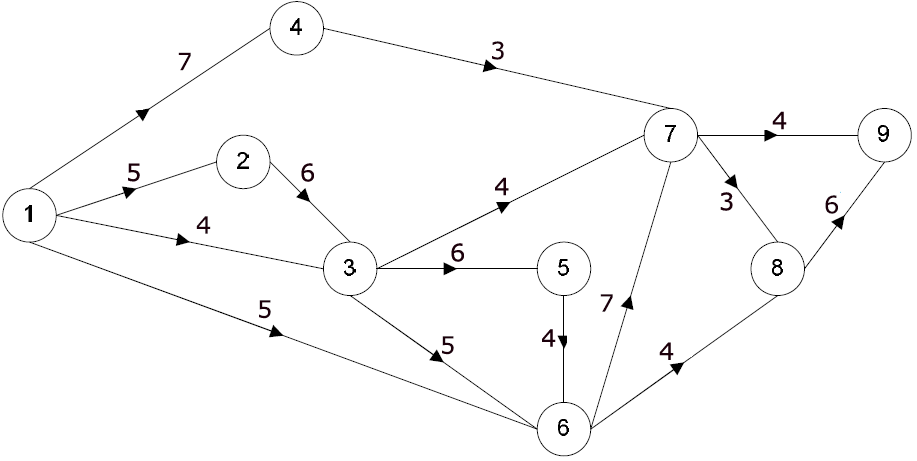
\includegraphics[width=1\linewidth]{img/00.png}}
\caption{Граф, описанный в задании по динамическому программированию}
\label{ris:image}
\end{figure}

\section{Решение. Часть 1}

\begin{table}[H]
\caption{Матрица смежности для заданного графа}
\label{tabular:timesandtenses}
\begin{center}
\begin{tabular}{|c|c|c|c|c|c|c|c|c|c|}
\hline
  & 0 & 1 & 2 & 3 & 4 & 5 & 6 & 7 & 8\\ \hline
0 & - & 5 & 4 & 7 & - & 5 & - & - & -\\ \hline
1 & - & - & 6 & - & - & - & - & - & -\\ \hline
2 & - & - & - & - & 6 & 5 & 4 & - & -\\ \hline
3 & - & - & - & - & - & - & 3 & - & -\\ \hline
4 & - & - & - & - & - & 4 & - & - & -\\ \hline
5 & - & - & - & - & - & - & 7 & 4 & -\\ \hline
6 & - & - & - & - & - & - & - & 3 & 4\\ \hline
7 & - & - & - & - & - & - & - & - & 6\\ \hline
8 & - & - & - & - & - & - & - & - & -\\ \hline
\end{tabular}
\end{center}
\end{table}

\newpage

Наиболее ранние моменты наступления событий:\\\\

\begin{minipage}{0.4\textwidth}
\begin{center}
 ${t_0}^{'} = 0$ \\
 ${t_1}^{'} = 5$ \\
 ${t_2}^{'} = 11$ \\
 ${t_3}^{'} = 7$ \\
 ${t_4}^{'} = 17$
\end{center}
\end{minipage}
\hfill
\begin{minipage}{0.5\textwidth}
\begin{center}
 ${t_5}^{'} = 21$ \\
 ${t_6}^{'} = 28$ \\
 ${t_7}^{'} = 31$ \\
 ${t_8}^{'} = 37$
\end{center}
\end{minipage}\\\\\\

Наиболее поздние моменты наступления событий:\\\\

\begin{minipage}{0.4\textwidth}
\begin{center}
 ${t_8}^{''} = 37$ \\
 ${t_7}^{''} = 31$ \\
 ${t_6}^{''} = 28$ \\
 ${t_5}^{''} = 21$ \\
 ${t_4}^{''} = 17$
\end{center}
\end{minipage}
\hfill
\begin{minipage}{0.5\textwidth}
\begin{center}
 ${t_3}^{''} = 25$ \\
 ${t_2}^{''} = 11$ \\
 ${t_1}^{''} = 5$ \\
 ${t_0}^{''} = 0$
\end{center}
\end{minipage}\\\\

\begin{table}[H]
\caption{Наиболее ранние/поздние моменты наступления событий}
\label{tabular:timesandtenses}
\begin{center}
\begin{tabular}{|c|c|c|c|c|c|c|c|c|c|}
\hline
  & 0 & 1 & 2 & 3 & 4 & 5 & 6 & 7 & 8\\ \hline
${t}^{'}$ & 0 & 5 & 11 & 7 & 17 & 21 & 28 & 31 & 37\\ \hline
${t}^{''}$ & 0 & 5 & 11 & 25 & 17 & 21 & 28 & 31 & 37\\ \hline
\end{tabular}
\end{center}
\end{table}

\begin{table}[H]
\caption{Матрица резервов}
\label{tabular:timesandtenses}
\begin{center}
\begin{tabular}{|c|c|c|c|c|c|c|c|c|c|}
\hline
  & 0 & 1 & 2 & 3 & 4 & 5 & 6 & 7 & 8\\ \hline
0 & - & 0 & 7 & 18 & - & 16 & - & - & -\\ \hline
1 & - & - & 0 & - & - & - & - & - & -\\ \hline
2 & - & - & - & - & 0 & 5 & 13 & - & -\\ \hline
3 & - & - & - & - & - & - & 18 & - & -\\ \hline
4 & - & - & - & - & - & 0 & - & - & -\\ \hline
5 & - & - & - & - & - & - & 0 & 6 & -\\ \hline
6 & - & - & - & - & - & - & - & 0 & 5\\ \hline
7 & - & - & - & - & - & - & - & - & 0\\ \hline
8 & - & - & - & - & - & - & - & - & -\\ \hline
\end{tabular}
\end{center}
\end{table}

\newpage

Критический путь: \ 1->2->3->5->6->7->8->9

Длина пути: \ 37

\begin{figure}[h]
\center{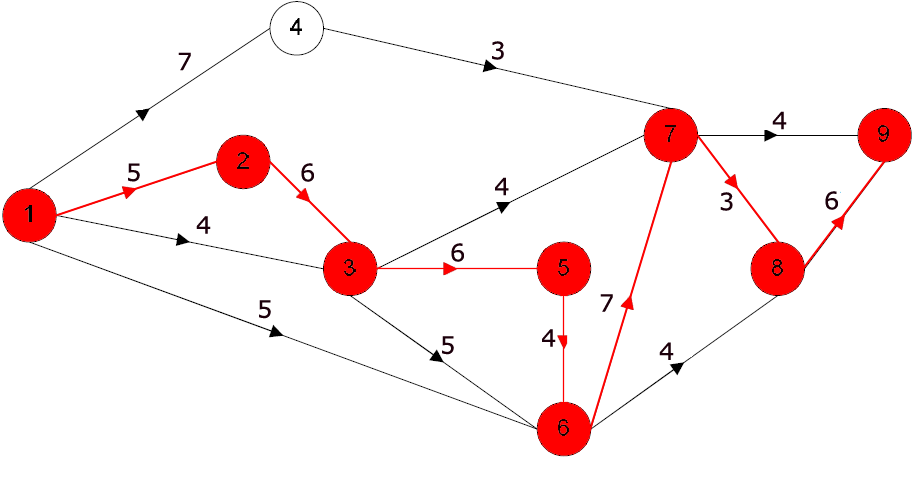
\includegraphics[width=1\linewidth]{img/01.png}}
\caption{Граф с выделенным критическим путём}
\label{ris:image}
\end{figure}

\section{Решение. Часть 2}

Допустим $N = 1$, тогда общее время выполнения будет равно сумме времени выполнения всех работ, т.е. $T = 73$ \\\\
Вариант 41, следовательно $N = 2$\\\\
T -- затраченное время \\
D -- законченные работы \\
E -- произошедшие события \\
W -- доступные работы \\
A -- длительность выполнения  \\
B -- выбранные для исполнения работы \\
L -- время, через которое окончится выполнение работы

\begin{table}[H]
\caption{Пошаговое выполнение при выборе работы с наибольшей длительностью исполнения}
\label{tabular:timesandtenses}
\begin{center}
\begin{tabular}{|c|c|c|c|c|c|c|}
\hline
T & D & E & W & A & B & L\\ \hline
0 & - & [0] & [0 1] [0 2] [0 3] [0 5] & [5 4 7 5] & [0 3] [0 1] & [7 5]\\ \hline
5 & [0 1] & [0 1] & [0 2] [0 5] [1 2] & [4 5 6] & [0 3] [1 2] & [2 6]\\ \hline
7 & [0 3] & [0 1 3] & [0 2] [0 5] [3 6] & [4 5 3] & [1 2] [0 5] & [4 5]\\ \hline
11 & [1 2] & [0 1 3] & [0 2] [3 6] & [4 3] & [0 5] [0 2] & [1 4]\\ \hline
12 & [0 5] & [0 1 3] & [3 6] & [3] & [0 2] [3 6] & [3 3]\\ \hline
15 & [0 2][3 6] & [0 1 2 3] & [2 4] [2 5] [2 6] & [6 5 4] & [2 4] [2 5] & [6 5]\\ \hline
20 & [2 5] & [0 1 2 3] & [2 6] & [4] & [2 4] [2 6] & [1 4]\\ \hline
21 & [2 4] & [0 1 2 3 4] & [4 5] & [4] & [2 6] [4 5] & [3 4]\\ \hline
24 & [2 6] & [0 1 2 3 4] &  - & - & [4 5] & [1]\\ \hline
25 & [4 5] & [0 1 2 3 4 5] & [5 6] [5 7] & [7 4] & [5 6] [5 7] & [7 4]\\ \hline
29 & [5 7] & [0 1 2 3 4 5] &  - & - & [5 6] & [3]\\ \hline
32 & [5 6] & [0 1 2 3 4 5 6] & [6 7] [6 8] & [3 4] & [6 8] [6 7] & [4 3]\\ \hline
35 & [6 7] & [0 1 2 3 4 5 6 7] & [7 8] & [6] & [6 8] [7 8] & [1 6]\\ \hline
36 & [6 8] & [0 1 2 3 4 5 6 7] &  - & - & [7 8] & [5]\\ \hline
41 & [7 8] & [0 1 2 3 4 5 6 7 8] &  - & - &  - & -\\ \hline
\end{tabular}
\end{center}
\end{table}

Общее время: 41

\begin{figure}[h]
\center{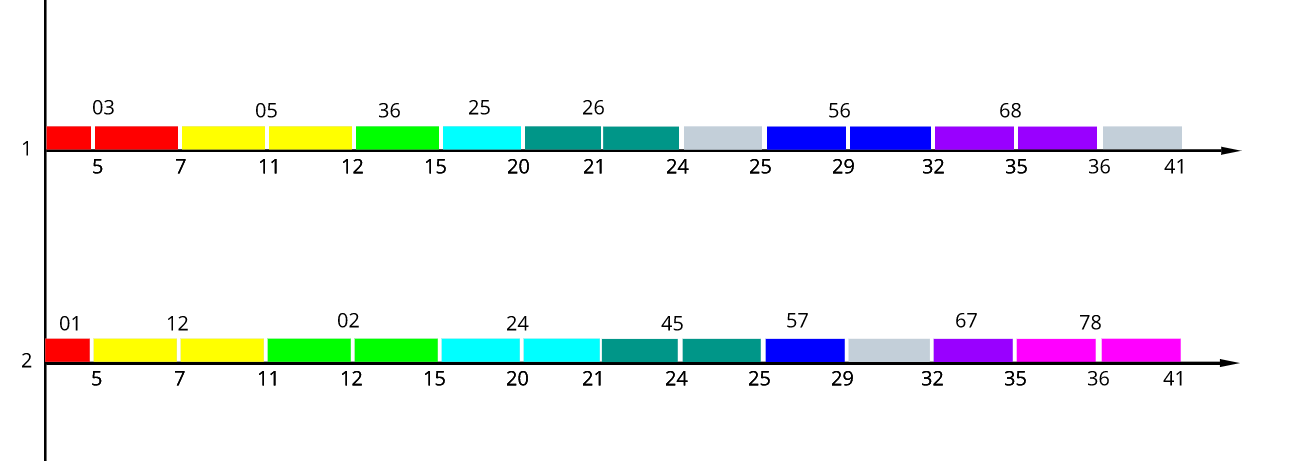
\includegraphics[width=1\linewidth]{img/img_tabl_1.png}}
\caption{Граф с выделенным критическим путём}
\label{ris:image}
\end{figure}

1-й простаивал 6 часов

2-й простаивал 3 часа

\begin{table}[H]
\caption{Пошаговое выполнение при выборе работы с наименьшей длительностью исполнения}
\label{tabular:timesandtenses}
\begin{center}
\begin{tabular}{|c|c|c|c|c|c|c|}
\hline
T & D & E & W & A & B & L\\ \hline
0 & - & [0] & [0 1]
 [0 2]
 [0 3]
 [0 5] & [5 4 7 5] & [0 2]
 [0 1] & [4 5] \\ \hline 
 4 & [0 2] & [0] & [0 3]
 [0 5] & [7 5] & [0 1]
 [0 5] & [1 5] \\ \hline 
 5 & [0 1] & [0 1] & [0 3]
 [1 2] & [7 6] & [0 5]
 [1 2] & [4 6] \\ \hline 
 9 & [0 5] & [0 1] & [0 3] & [7] & [1 2]
 [0 3] & [2 7] \\ \hline 
 11 & [1 2] & [0 1 2] & [2 4]
 [2 5]
 [2 6] & [6 5 4] & [0 3]
 [2 6] & [5 4] \\ \hline 
 15 & [2 6] & [0 1 2] & [2 4]
 [2 5] & [6 5] & [0 3]
 [2 5] & [1 5] \\ \hline 
 16 & [0 3] & [0 1 2 3] & [2 4]
 [3 6] & [6 3] & [2 5]
 [3 6] & [4 3] \\ \hline 
 19 & [3 6] & [0 1 2 3] & [2 4] & [6] & [2 5]
 [2 4] & [1 6] \\ \hline 
 20 & [2 5] & [0 1 2 3] & - & - & [2 4] & [5] \\ \hline 
 25 & [2 4] & [0 1 2 3 4] & [4 5] & [4] & [4 5] & [4] \\ \hline 
 29 & [4 5] & [0 1 2 3 4 5] & [5 6]
 [5 7] & [7 4] & [5 7]
 [5 6] & [4 7] \\ \hline 
 33 & [5 7] & [0 1 2 3 4 5] & - & - & [5 6] & [3] \\ \hline 
 36 & [5 6] & [0 1 2 3 4 5 6] & [6 7]
 [6 8] & [3 4] & [6 7]
 [6 8] & [3 4] \\ \hline 
 39 & [6 7] & [0 1 2 3 4 5 6 7] & [7 8] & [6] & [6 8]
 [7 8] & [1 6] \\ \hline 
 40 & [6 8] & [0 1 2 3 4 5 6 7] & - & - & [7 8] & [5] \\ \hline 
 45 & [7 8] & [0 1 2 3 4 5 6 7 8] & - & - & - & - \\ \hline 
\end{tabular}
\end{center}
\end{table}

Общее время: 45

\begin{figure}[h]
\center{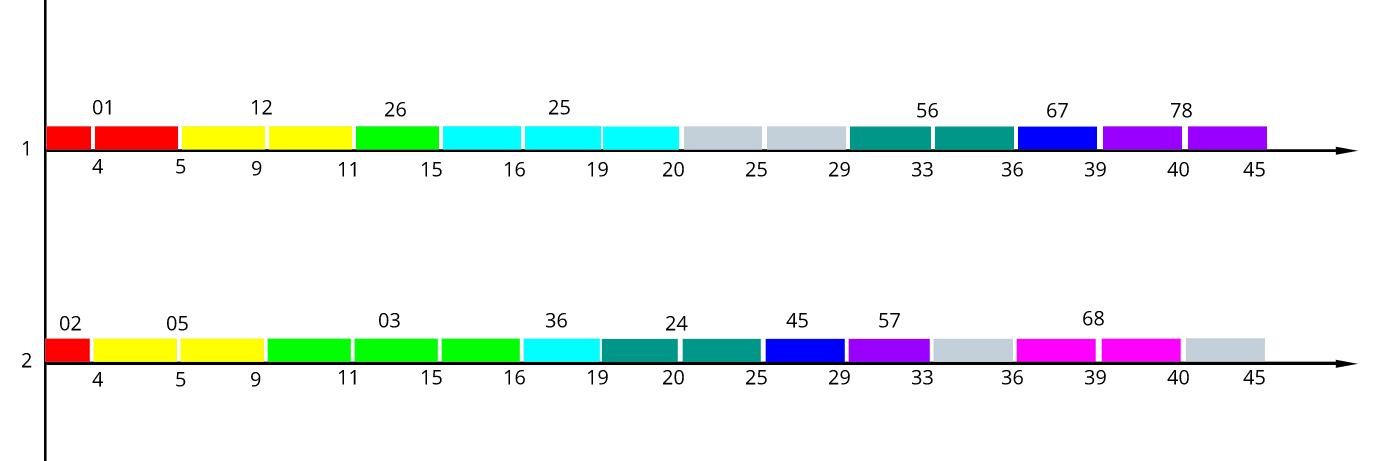
\includegraphics[width=1\linewidth]{img/img_tabl_2.png}}
\caption{Граф с выделенным критическим путём}
\label{ris:image}
\end{figure}

1-й простаивал 9 часов

2-й простаивал 8 часа

\begin{table}[H]
\caption{Пошаговое выполнение при выборе работы с наименьшим резервом}
\label{tabular:timesandtenses}
\begin{center}
\begin{tabular}{|c|c|c|c|c|c|c|}
\hline
T & D & E & W & A & B & L\\ \hline
0 & - & [0] & [0 1]
 [0 2]
 [0 3]
 [0 5] & [5 4 7 5] & [0 1]
 [0 2] & [5 4] \\ \hline 
 4 & [0 2] & [0] & [0 3]
 [0 5] & [7 5] & [0 1]
 [0 5] & [1 5] \\ \hline 
 5 & [0 1] & [0 1] & [0 3]
 [1 2] & [7 6] & [0 5]
 [1 2] & [4 6] \\ \hline 
 9 & [0 5] & [0 1] & [0 3] & [7] & [1 2]
 [0 3] & [2 7] \\ \hline 
 11 & [1 2] & [0 1 2] & [2 4]
 [2 5]
 [2 6] & [6 5 4] & [0 3]
 [2 4] & [5 6] \\ \hline 
 16 & [0 3] & [0 1 2 3] & [2 5]
 [2 6]
 [3 6] & [5 4 3] & [2 4]
 [2 5] & [1 5] \\ \hline 
 17 & [2 4] & [0 1 2 3 4] & [2 6]
 [3 6]
 [4 5] & [4 3 4] & [2 5]
 [4 5] & [4 4] \\ \hline 
 21 & [2 5]
 [4 5] & [0 1 2 3 4 5] & [2 6]
 [3 6]
 [5 6]
 [5 7] & [4 3 7 4] & [5 6]
 [5 7] & [7 4] \\ \hline 
 25 & [5 7] & [0 1 2 3 4 5] & [2 6]
 [3 6] & [4 3] & [5 6]
 [2 6] & [3 4] \\ \hline 
 28 & [5 6] & [0 1 2 3 4 5] & [3 6] & [3] & [2 6]
 [3 6] & [1 3] \\ \hline 
 29 & [2 6] & [0 1 2 3 4 5] & - & - & [3 6] & [2] \\ \hline 
 31 & [3 6] & [0 1 2 3 4 5 6] & [6 7]
 [6 8] & [3 4] & [6 7]
 [6 8] & [3 4] \\ \hline 
 34 & [6 7] & [0 1 2 3 4 5 6 7] & [7 8] & [6] & [6 8]
 [7 8] & [1 6] \\ \hline 
 35 & [6 8] & [0 1 2 3 4 5 6 7] & - & - & [7 8] & [5] \\ \hline 
 40 & [7 8] & [0 1 2 3 4 5 6 7 8] & - & - & - & - \\ \hline 
\end{tabular}
\end{center}
\end{table}

Общее время: 40

\begin{figure}[h]
\center{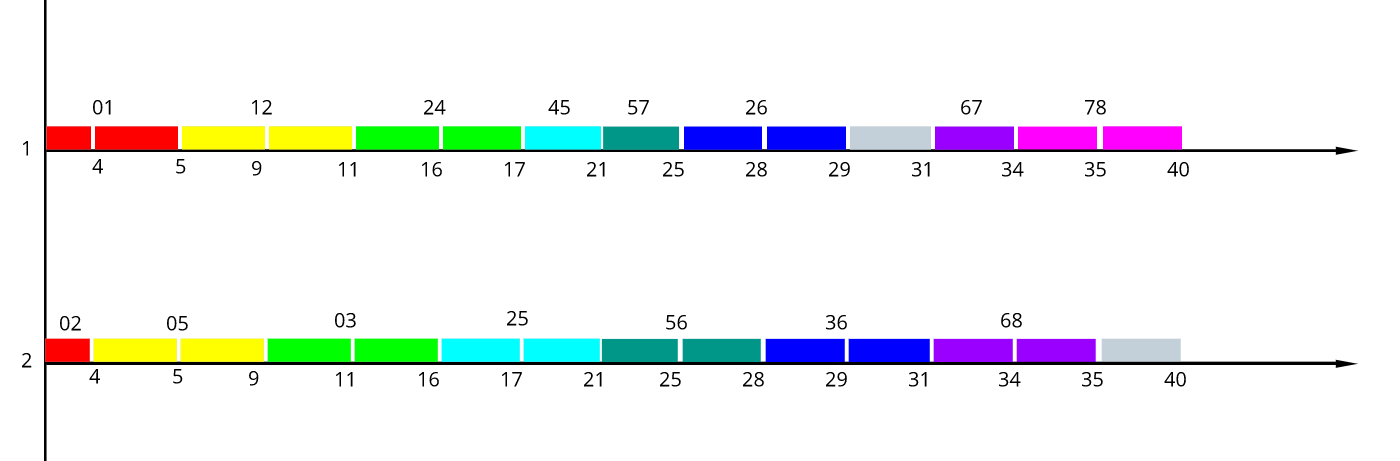
\includegraphics[width=1\linewidth]{img/img_tabl_3.png}}
\caption{Граф с выделенным критическим путём}
\label{ris:image}
\end{figure}

1-й простаивал 2 часов

2-й простаивал 5 часа

\begin{table}[H]
\caption{Пошаговое выполнение при выборе работы с наибольшим резервом}
\label{tabular:timesandtenses}
\begin{center}
\begin{tabular}{|c|c|c|c|c|c|c|}
\hline
T & D & E & W & A & B & L\\ \hline
0 & - & [0] & [0 1]
 [0 2]
 [0 3]
 [0 5] & [5 4 7 5] & [0 3]
 [0 5] & [7 5] \\ \hline 
 5 & [0 5] & [0] & [0 1]
 [0 2] & [5 4] & [0 3]
 [0 2] & [2 4] \\ \hline 
 7 & [0 3] & [0 3] & [0 1]
 [3 6] & [5 3] & [0 2]
 [3 6] & [2 3] \\ \hline 
 9 & [0 2] & [0 3] & [0 1] & [5] & [3 6]
 [0 1] & [1 5] \\ \hline 
 10 & [3 6] & [0 3] & - & - & [0 1] & [4] \\ \hline 
 14 & [0 1] & [0 1 3] & [1 2] & [6] & [1 2] & [6] \\ \hline 
 20 & [1 2] & [0 1 2 3] & [2 4]
 [2 5]
 [2 6] & [6 5 4] & [2 6]
 [2 5] & [4 5] \\ \hline 
 24 & [2 6] & [0 1 2 3] & [2 4] & [6] & [2 5]
 [2 4] & [1 6] \\ \hline 
 25 & [2 5] & [0 1 2 3] & - & - & [2 4] & [5] \\ \hline 
 30 & [2 4] & [0 1 2 3 4] & [4 5] & [4] & [4 5] & [4] \\ \hline 
 34 & [4 5] & [0 1 2 3 4 5] & [5 6]
 [5 7] & [7 4] & [5 7]
 [5 6] & [4 7] \\ \hline 
 38 & [5 7] & [0 1 2 3 4 5] & - & - & [5 6] & [3] \\ \hline 
 41 & [5 6] & [0 1 2 3 4 5 6] & [6 7]
 [6 8] & [3 4] & [6 8]
 [6 7] & [4 3] \\ \hline 
 44 & [6 7] & [0 1 2 3 4 5 6 7] & [7 8] & [6] & [6 8]
 [7 8] & [1 6] \\ \hline 
 45 & [6 8] & [0 1 2 3 4 5 6 7] & - & - & [7 8] & [5] \\ \hline 
 50 & [7 8] & [0 1 2 3 4 5 6 7 8] & - & - & - & - \\ \hline 
\end{tabular}
\end{center}
\end{table}

Общее время: 50\\\\

\begin{figure}[h]
\center{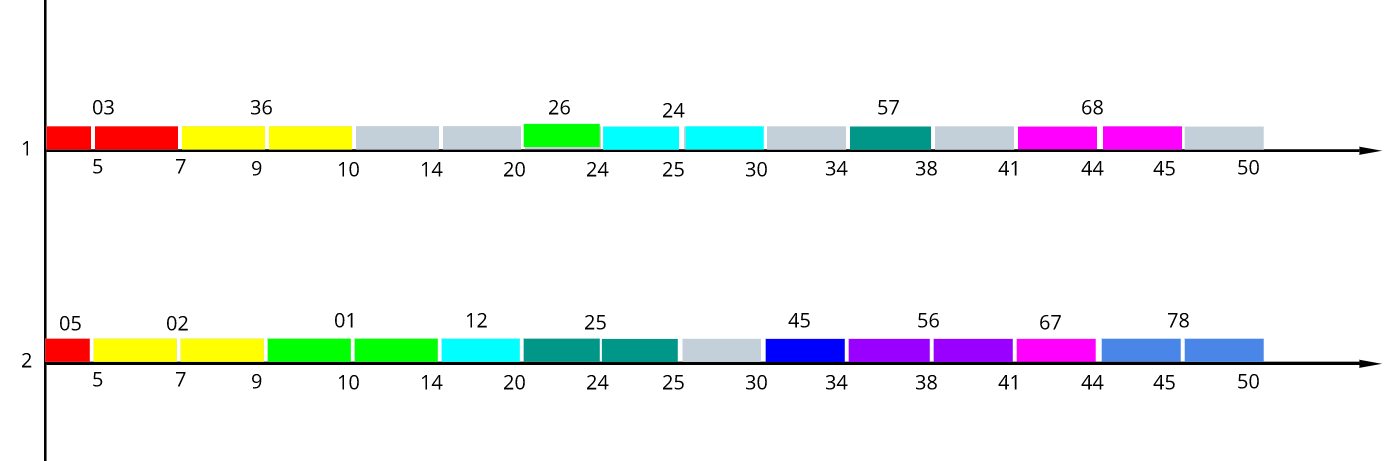
\includegraphics[width=1\linewidth]{img/img_tabl_4.png}}
\caption{Граф с выделенным критическим путём}
\label{ris:image}
\end{figure}

1-й простаивал 22 часов

2-й простаивал 5 часа


\section{Вывод}

Лучший критерий выбора -- выбор работы с наименьшим резервом\\
Наименьшая длительность выполнения работ, при 2-х рабочих: 40


\end{document}
